
\subsection{Konvertering af DTM til DHyM} \label{Sektion: Konvertering af DTM til DHyM}
Et vigtigt element af en realistisk oversvømmelsesmodellering er at kunne simulere korrekt hydrologisk adfærd gennem terrænet. Det er derfor essentielt for at kunne bruge modellens resultater tillidsfuldt at den digitale terrænmodel (DTM) bliver korrigeret og konverteret til en digital hydrologisk model (DHyM).\\ 

For at konvertere en DTM til DHyM bliver der anvendt to geometrisk dataobjekter: Linje- og hesteskotilpasninger. Begge objekter er linjeobjekter og bliver brændt ned i DTM for at simulere korrekt geografiske karakteristika i landskabet, som ikke er blevet fanget af højdemodellen. \\
Da der findes tilpasninger for både simuleringer af skybrud og stormfloder, er det vigtigt at der kun bliver anvendt de tilpasninger der har indflydelse på havstigningsmodellering. Det vil derfor betyde at der ikke skal inkluderes tilpasninger, som er designet til at føre regnvand fra skybrud ud i havet. Tilpasninger såsom skybrudskontraklappe er derfor blevet fravalgt. Der er derfor lavet en selektering af de korrekte tilpasninger i databasen for hvert område.\\

Dette er gjort for både linje- og hesteskotilpasningerne ved brug af værktøjet \textit{"Extract Hydroconditoning Inundation"}, som laver en søgning i databaserne for tilpasningslagene. Først søger værktøjet efter alle tilpasninger indenfor studieområdet defineret ud fra en maske. Herefter laves der en søgning i attributtabellen for en anvendelses beskrivelse. Til stormflodsmodellering skal der anvendes tre attributter og deres funktionalitet er beskrevet i tabel \ref{Tabel: Relevante hydrologiske tilpasninger}. De tilpasninger som opfylder én af kriterierne bliver overført til et nyt lag, en for linjetilpasninger og en for hesteskotilpasninger.  

\begin{table}[H]
\centering
\renewcommand{\arraystretch}{1.5}
\begin{threeparttable}
\caption{Relevante hydrologiske tilpasninger. Kilde: \cite{GeoDanmark_HydroLag}}
\label{Tabel: Relevante hydrologiske tilpasninger}
\begin{tabular}{@{} l l @{}} 
\toprule
\textbf{Navn} & \textbf{Beskrivelse} \\
\midrule
\textit{Generel} &
  \makecell[l]{Den normale tilpasning af hydrologiske forhold\\
  (fx skabelse af et frit forløb under en bro)} \\
\addlinespace
\textit{Havstigning} &
  \makecell[l]{Tilpasninger der skal forhindre, at vand løber ind\\
  over det bagvedliggende land\\
  (fx lukning af en højvandssluse)} \\
\addlinespace
\textit{DHMFix} &
  \makecell[l]{Bruges ved ændringer, der har hydrologisk effekt\\
  på vandets frie forløb på terrænoverfladen\\
  (fx reparation af fejl i den specifikke DHM)} \\
\bottomrule
\end{tabular}
\end{threeparttable}
\end{table}

Inden tilpasningerne bliver brændt ned i DTM, skal hesteskotilpasningerne ændres fra deres hesteskoform til at have en række linje mellem ydrekanterne af hesteskoen. Dette gøres for at få den præcise størrelse og udbredelse af tilpasningen brændt ned i DTM fremfor for omridset af tilpasningen. Det er blevet gjort ved at bruge et Python-script \textit{"Convert Horsehoes to Lines"} hvor både linje- og hesteskotilpasningerne fundet i \textit{"Extract Hydroconditioning Inundation"} bliver omdannet til separate linjer. Ved at konvertere hesteskotilpasningerne til separate linjer er det muligt at brænde tilpasningens korrekt form ned i DTM, da hesteskotilpasningernes originale form ikke er egnet til at blive brændt ned i DTM. \\
Linjerne til hesteskotilpasningerne bliver defineret ud fra de 4 hjørnepunkter af hesteskoen og cellestørrelsen af DTM. Ændringen af hesteskotilpasningen til linjer er vist i \ref{Figur: Ændringen af hesteskotilpasningerne}. Hvor figur \ref{Subfig: Hesteskotilpasninger før ændring} er tilpasningen før ændring og figur \ref{Subfig: Hesteskotilpasning efter tilpasningen er konverteret til linjer} er tilpasningen efter den er blevet konverteret til separate linjer. Hver linje er præcis en cellestørrelse bred, da det ikke er nødvendigt at have en større linjebredde for at simulere korrekt hydrologisk bevægelse igennem terrænet. 

\begin{figure}[H]
    \begin{subfigure}[t]{0.5\textwidth}
        \centering
        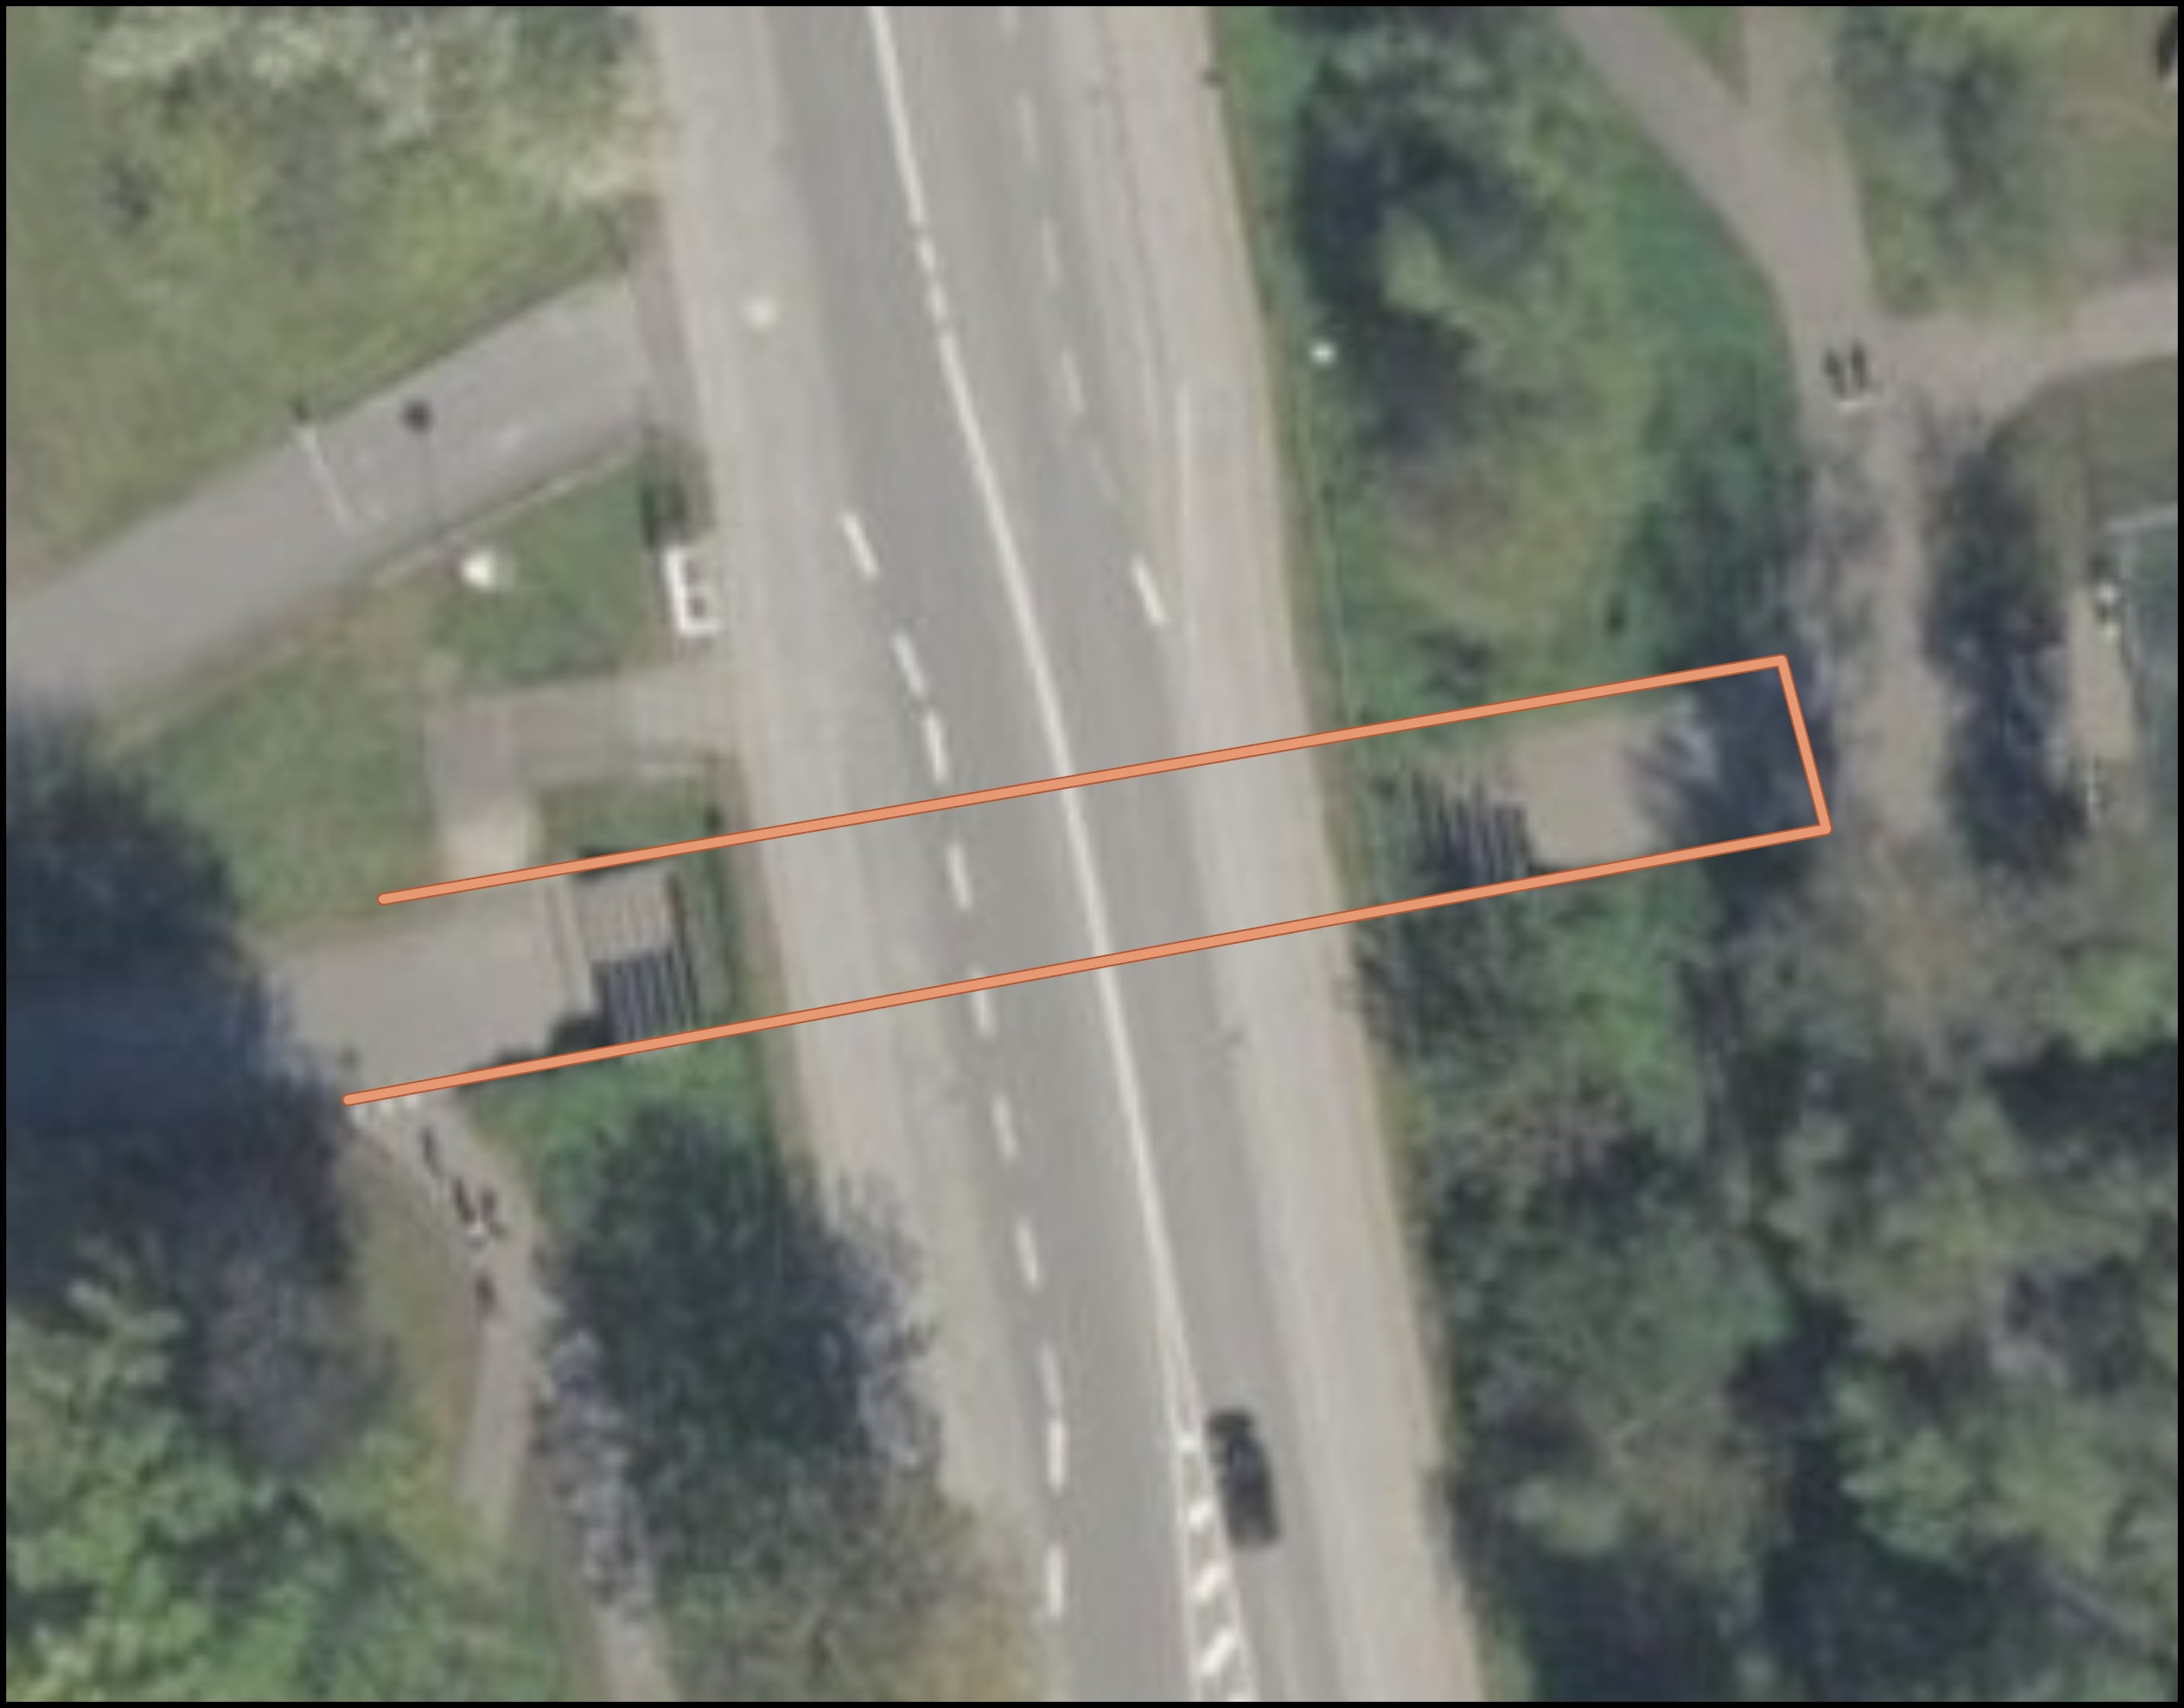
\includegraphics[width=1\linewidth]{images/databeskrivelse/hestesko.jpg}
        \caption{}
        \label{Subfig: Hesteskotilpasninger før ændring}
    \end{subfigure}
    \hspace{0.2cm}
    \begin{subfigure}[t]{0.5\textwidth}
        \centering
        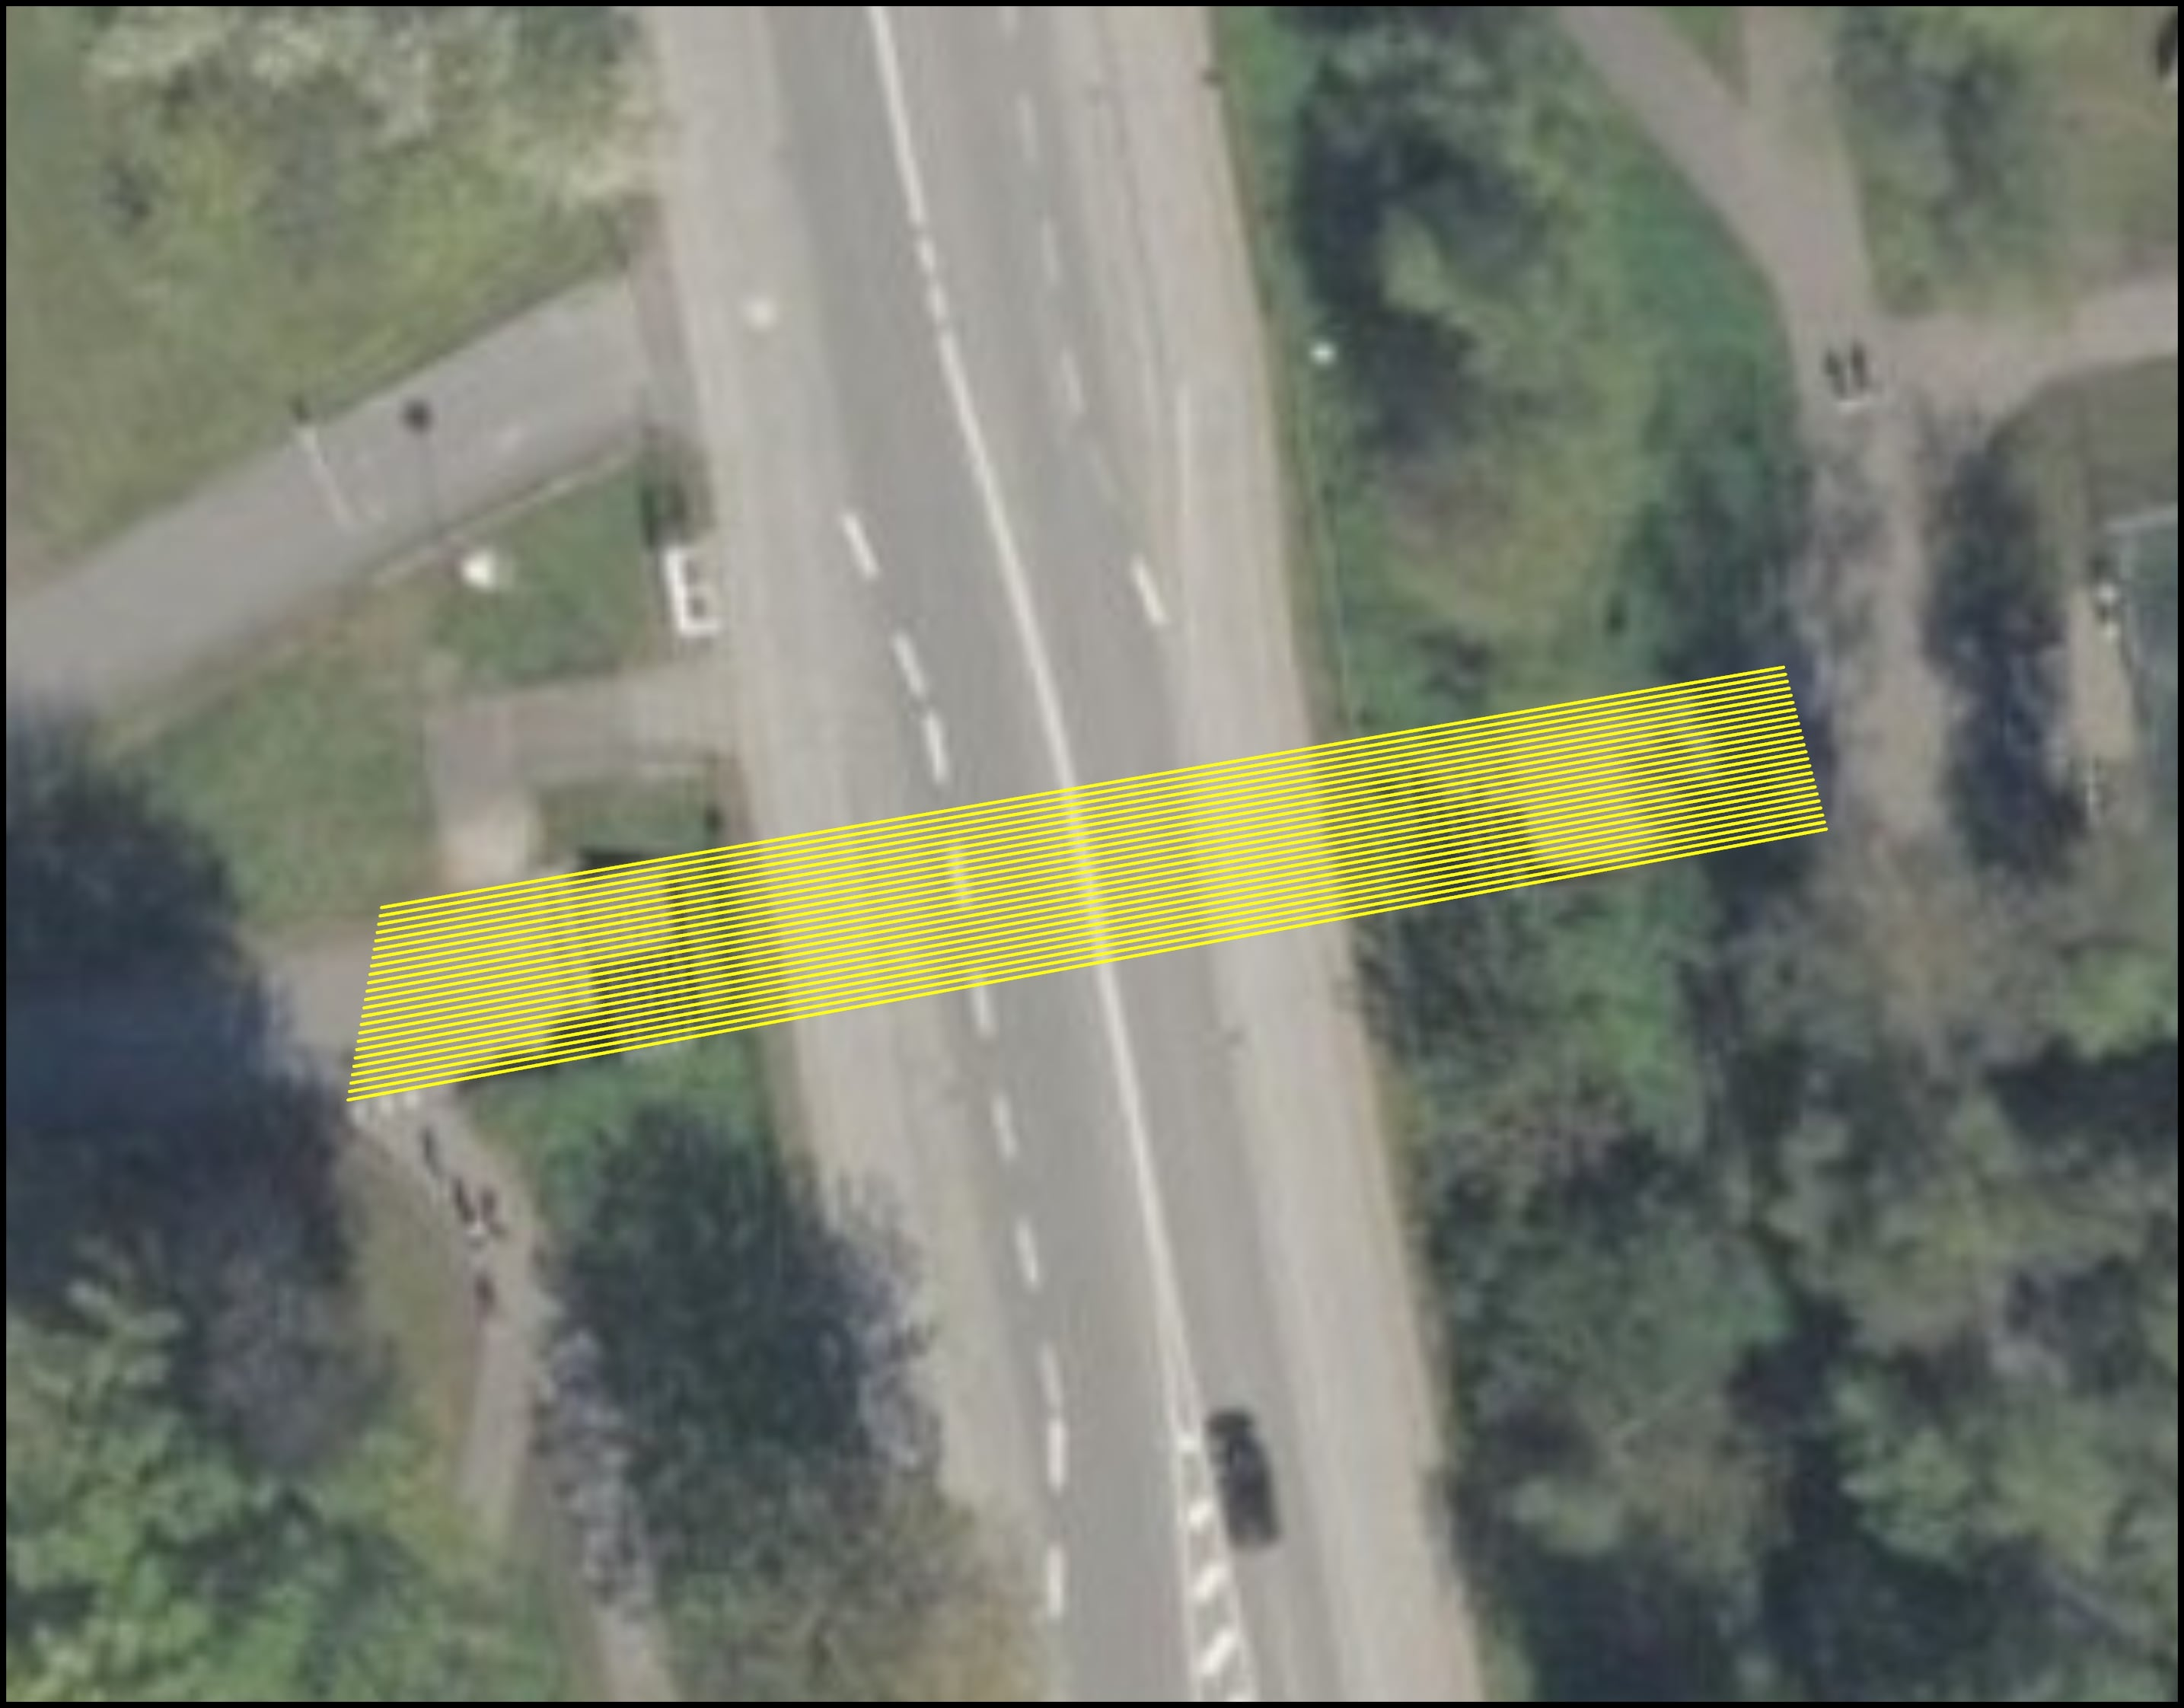
\includegraphics[width=1\linewidth]{images/metode/hestesko_linjer.jpg}
        \caption{}
        \label{Subfig: Hesteskotilpasning efter tilpasningen er konverteret til linjer}
    \end{subfigure}
    \caption{Ændringen af hesteskotilpasningerne fra en hesteskoform til separate linjer. \textbf{(a)} Hesteskotilpasninger før ændring \textbf{(b)} Hesteskotilpasning efter tilpasningen er konverteret til linjer}
    \label{Figur: Ændringen af hesteskotilpasningerne}
\end{figure}

Dette skaber et nyt sammenlagt lag med alle de relevante hydrologiske tilpasninger som linjer der blev brændt ned i DTM. For at tilpasningen bliver korrekt repræsenteret i DHyM skal højdeværdier under terræn hindringen først interpoleres.\\
Dette blev gjort ved at bruge et Python-script \textit{"Hydrologic Conditioning Multiple"}, som tildeler en z-værdi fra DTM til linjernes endepunkter: $Z_0$ og $Z_1$. Ud fra linjernes endepunkter bliver linjens hældning, $\Delta{Z}$ udregnet ved at bruge linjens længde. Linjen konverteres til et rasterformat og derefter til punkter for hver celle i DTM, hvor der laves en lineær interpolation af punkterne på linjen baseret på startpunktet $Z_0$, afstanden fra $Z_0$ til punktet og linjetilpasningens hældning, $\Delta{Z}$. Dette gøres for alle punkter langs linjen (figur \ref{Figur: Interpolation af Z-værdier}). \\
Efter punkterne er blevet interpoleret, konverteres der tilbage til et rasterformat, hvorefter de hydrologiske tilpasninger brændes ned i DTM ved at kombinere rasteren med de interpoleret punkter og DTM. Dette skaber den korrigeret Digitale Hydrologiske Model (DHyM).

\begin{figure}[H]
    \centering
    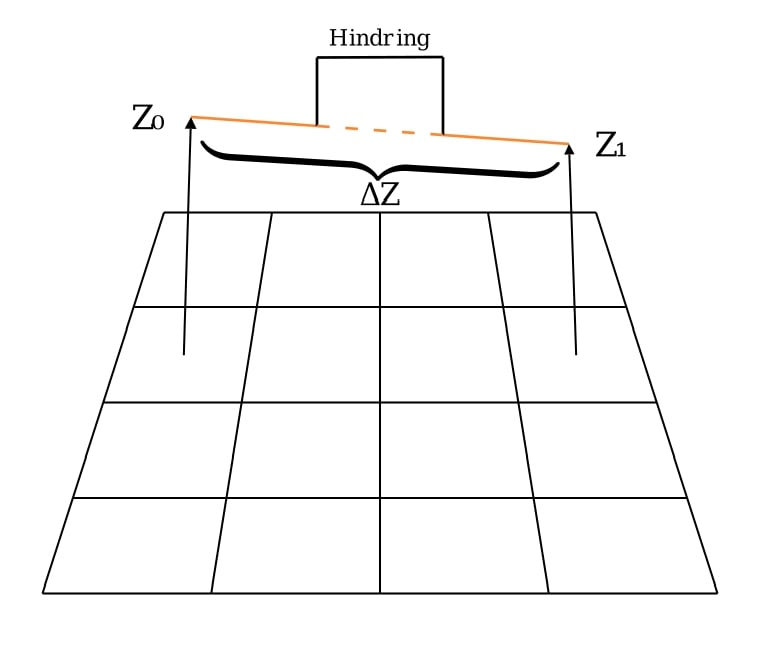
\includegraphics[width=0.5\linewidth]{images/metode/dtm_hydro_z.jpg}
    \caption{Interpolationen af z-værdier for en linjetilpasning under en hindring. $Z_1$ og $Z_0$ er z-værdierne fra DTM ved linjetilpasningens endepunkter og $\Delta{Z}$ er hældningen af linjetilpasningen. Egen illustration med inspiration fra \cite{balstrom_identification_2024}}
    \label{Figur: Interpolation af Z-værdier}
\end{figure}

For studieområderne Aabenraa, Gedser Havn, Hesnæs og Præstø blev der identificeret henholdsvis 250, 13, 34 og 19 hydrologiske tilpasninger, som blev brændt ned i deres tilhørende DTM.


\subsubsection{Inklusion af bygninger i DHyM} \label{Afsnit: Inklusion af bygninger i DHyM}

Efter de hydrologiske tilpasninger blev brændt ned i DTM, blev der besluttet at inkludere bygninger i DHyM, som en ikke-gennemtrængelige barrierer i terrænet. Denne beslutning blev truffet med udgangspunkt i, at de oversvømmelseskort studiekommunerne havde leveret, behandlede bygninger som barrierer. Desuden blev det vurderet at en realistisk simulering af hydrologisk adfærd forudsætter, at vand ikke kan strømme igennem bygninger, men ledes udenom. \\

Metoden for at implementere bygninger i DHyM blev gennemført ved brug af \textit{"Building Block (BB)"} metoden anvendt i \cite{khosh_bin_ghomash_technical_2024} ved at hæve terrænhøjden for hver bygningspolygoners fodaftryk til en bestemt højde. Denne højde blev arbitrært sat til 20 meter for alle bygningerne. Herefter blev bygningspolygonerne konverteret til et rasterformat med den samme cellestørrelse på 40\times40 cm som DHyM. \\
Derefter udføres der et tjek på den nye raster med bygningerne, hvor celler med værdien 20 forblev 20 og celler med NoData blev tildelt værdien 0. Dette sikrer at bygningsrasteren kan kombineres med DHyM, da beregninger på NoData-værdier ikke er mulige. Til sidst blev bygningsrasteren og DHyM lagt sammen, hvilket skabte den endelige DHyM, som anvendes i Inundation Modellen.


\subsection{Simulering af oktober 2023 stormfloden}\label{Afsnit: Simulering af stormflod 2023}

Efter DTM er blevet konverteret til en DHyM er det muligt at udføre stormflodsmodellering via Inundation Modellen. I modellen inputtes der for hvert studieområde den tilhørende DHyM og kildelinjen \textit{"Line at Sea"}. Line At Sea linjen er manuelt digitaliseret i hvert studieområde ude i havet.\\ Hvert studieområde simuleres op til det højeste officielle vandstandsniveau målt ved oktober 2023 stormfloden og antallet af iterationer for at opnå dette niveau er vist i tabel \ref{Tabel: Antal iterationer og slutværdier for Inundation Model}. Alle studieområder starter oversvømmelsessimuleringen med værktøjet \textit{"Create Inundation"} fra  100 cm og en vandstandsstigningsværdi på 1 cm. En startværdi på 100 cm blev valgt på baggrund af processeringstid og vandstandsstigningsværdien på 1 cm blev valgt for at opnå størst fleksibilitet og for at få nøjagtig samme vandstandsniveau som målt under stormfloden den 20. oktober 2023. Simuleringstiden for hver af de fire studieområder er vist i tabel \ref{Tabel: Antal iterationer og slutværdier for Inundation Model} og sammenlagt tog det 12 timer og 1 minut at simulere oktober 2023 stormfloden ved brug af Inundation Modellen på de fire studieområder.  \\
\begin{table}[H]
\centering
\renewcommand{\arraystretch}{1}
\begin{threeparttable}
\caption{Antal iterationer, slutværdien og processeringstiden for oversvømmelsessimuleringer i Inundation Modellen for simulere oktober 2023 stormfloden}
\begin{tabular}{@{} l 
                S[table-format=7.2, output-decimal-marker={,}] 
                S[table-format=7.2, output-decimal-marker={,}]
                l @{}} 
\toprule
\textbf{Lokalitet} & \textbf{Antal iterationer} & \textbf{Slutværdi (cm)}  & \textbf{Simuleringstid}\\
\midrule
Aabenraa & 117 & 216 & 5 timer 27 minutter \\
Gedser & 90 & 189 & 3 timer 25 minutter\\ 
Hesnæs & 111 & 210 & 1 time 23 minutter \\
Præstø & 101 & 200 & 1 time 44 minutter \\
\bottomrule
\end{tabular}
\label{Tabel: Antal iterationer og slutværdier for Inundation Model}
\end{threeparttable}
\end{table}

Efter simuleringen er gennemført er der produceret tre rasterlag, et "Inundation", "Backdirection", og "Distance Accumulation" -lag, for hver cm fra startværdien på 100 til slutværdien for hvert område. Ved brug af det interne ArcGIS Pro værktøj \textit{"Cell Statistics"} blev "Inundation" \hspace{0.2cm} lagene fra 100 cm til slutværdien for det givne studieområde kombineret ved at finde minimum oversvømmelseværdi af hver celle. Her er der blevet brugt en landpolygon til at filtrere resultatet, så det kun er oversvømmelsen på land der er visualiseret. Dette producerer et samlet kort over oversvømmelsen simuleret af Inundation Modellen der kan sammenlignes med de modtaget kort over vandets udbredelse fra studiekommunerne. 

\subsection{Kvantificering af påvirkede areal anvendelser} \label{Afsnit: Udregning af påvirkede areal anvendelser}

Til at kvantificere påvirkningen 2023 stormfloden havde på studieområderne blev der gennemført en krydstabulering mellem arealanvendelsesklasserne fra BaseMap04 og både den observeret og simuleret oversvømmelse af stormfloden. \\

Først blev BaseMap04-arealanvendelsesrasteren, der oprindeligt har en cellestørrelse på 10\times10 m, resamplet til en cellestørrelse svarende til outputtet fra Inundation Modellen (40\times40 cm). Derefter blev værktøjet \textit{"Tabulate Area"} anvendt til at beregne det oversvømmede areal for hver arealanvendelsesklasse, både for den observerede stormflod og for resultaterne fra Inundation Modellen. 
\begin{figure}[H]
    \centering
    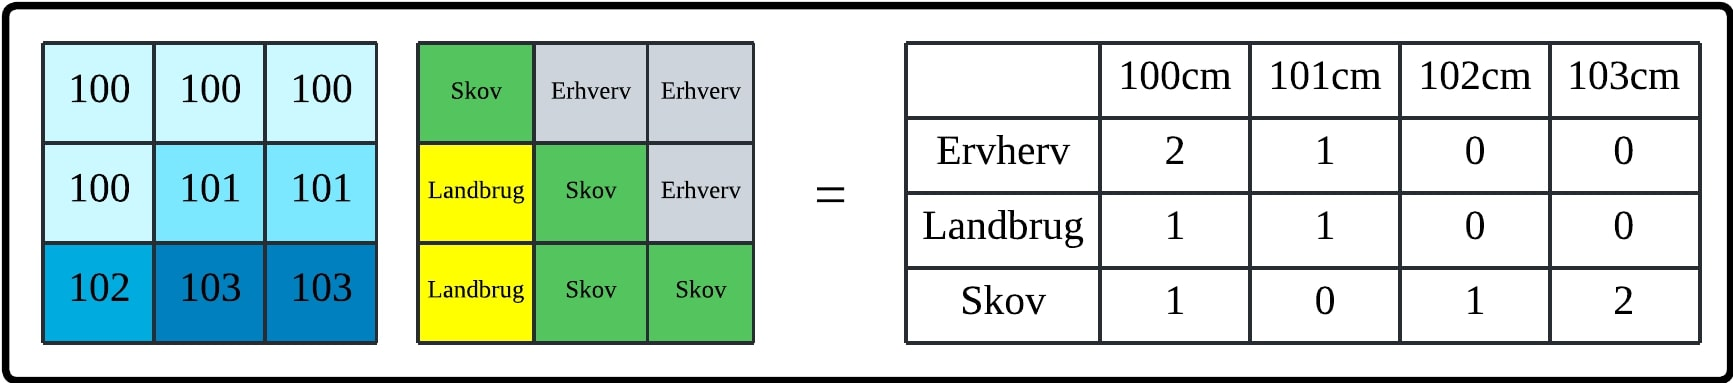
\includegraphics[width=1\linewidth]{images/metode/tabulate.jpg}
    \caption{Krydstabulerings processen bag Tabulate Area værktøjet i ArcGIS Pro. Hver celle i oversvømmelsesrasteren kobles til en celle i arealanvendelsesrasteren og tabuleres. Egen illustration med inspiration fra \cite{esri_tabulate_nodate}}
    \label{Figur: Tabulate}
\end{figure}
Værktøjet Tabulate Area krydsreferer hver celle i BaseMap-arealanvendelsesrasteren med den tilsvarende celle i oversvømmelsesrasteren så der bliver knyttet en arealanvendelse til et oversvømmelsesniveau, der muliggør en rumlig kvantificering af stormflodens påvirkning på arealanvendelserne i studieområderne (figur \ref{Figur: Tabulate}).\\

Resultatet af krydstabuleringen præsenteres som en kontingenstabel med arealklasserne som rækker og hvert oversvømmelsesniveau i centimeter som kolonner. På baggrund af denne tabel summeres antallet af celler for hver unikke arealanvendelsesklasse, hvorefter det påvirkede areal for hver arealklasse beregnes som andel af det samlede oversvømmede areal og visualiseres som et søjlediagram. 

\subsection{Fremskrivning af 2023 stormfloden og en statistisk 100-års hændelse} \label{Afsnit: Fremskrivning og statistisk}

Til at undersøge hvordan studieområderne vil blive påvirket i lyset af fremtidige klimaforandringer især af risikoen for stigende vandstand. Til dette er der blevet undersøgt to forskellige metoder til at undersøge påvirkningen af klimaforandringer: et statistisk oversvømmelsesniveau ved en 100-års hændelse som præsenteret af Klimaatlas fra \cite{dmi_data_2025} og en fremskrivning af oktober 2023 stormfloden til slutningen af det nuværende århundrede baseret på projektioner fra den sjette \cite{ipcc_report_AR6} rapport.\\

{\large \textit{Statistisk 100-års hændelse}}\\
For at undersøge påvirkningen af studieområderne baseret på en statistisk 100-års hændelse, blev DMIs Klimaatlas anvendt til at bestemme vandstandshøjden af en stormflod der statistisk set vil optræde en gang per 100 år. Klimaatlas inddeler Danmarks kyster i kyststrækninger og de fire kyststrækninger der blev anvendt er: Lillebælt Syd for Aabenraa, Femern Bælt for Gedser, Falsters og Møns Østersøkyst for Hesnæs og Faxe Bugt for Præstø. For hver kyststrækning bruges den absolute vandstandshøjde for en statistisk 100-års hændelse ved to Shared Socioeconomic Pathways (SSP) scenarie: et mellemhøjt udledningsscenarie (SSP2,5-4,5) og et meget højt udledningsscenarie (SSP5-8,5). \\
Herefter bruges Inundation Modellen til at simulere op til SSP5-8,5 scenariet for hvert studieområde. Processen bag dette er den samme som i afsnit \ref{Afsnit: Simulering af stormflod 2023}, men i stedet for at starte ved 100 cm starter modellen ved den observerde vandstandshøjde ved stormfloden for hvert studieområde. Der blev simuleret op til en vandstandshøjde på 251 cm for Aabenraa, 242 cm for Gedser, 253 cm for Hesnæs og 225 cm for Præstø og tilføjede sammenlagt en ekstra 2 timer og 46 minutter i simuleringstid. \\

{\large \textit{Fremskrivning}} \\
Til at fremskrive hvordan oktober 2023 stormfloden vil se ud i slutningen af det nuværende århundrede på baggrund af stigende havspejl blev der lavet en udregning af middelvandstanden i slutningen af århundredet. DMIs Klimaatlas har allerede tal for middelvandstanden i slutningen af århundredet, men de er i forhold til en referenceperiode fra 1981-2010. Det har derfor været nødvendigt at finde middelvandstandsniveauet i 2023 i forhold til DMIs referenceperiode. \\

Til udregningen af dette er der blev der brugt et værktøj udarbejdet af \cite{NASA_tool} til at få havspejlsstignings projektioner fra \cite{garner_ipcc_2021} til en bestemt Permanent Service for Mean Sea Level (PSMSL) station. I værktøjet vælges der den nærmeste PSMSL station for hvert studieområde. PSMSL stationen blev udvalgt ud fra det hav basin der var tættest på hvert studieområde. Dette var Fynshav for Aabenraa, Gedser Havn for Gedser, Warnemünde for Hesnæs og Skanör for Præstø.\\

Værktøjet giver derefter en tabel med alle de individuelle bidrag til havspejlsstigning og en median havspejlsstigning ($SLR_{50}$) for hver station i forhold til en referenceperiode fra 1995-2014. $SLR_{50}$ indeholder en række faktorer der påvirker havspejlsstigning, såsom ferskvandstilførsel fra floder, glacial bidrag og tager højde for lokal isostasi. For at udregne middelvandstanden i 2023, er projektionen for 2030 anvendt, da det er den tætteste. Til udregningen er der blevet opstillet en følgende ligning: 
\begin{align} \label{Equation: Vandstandsstigning calculation}
    S_r = S_p- \left( \frac{\Delta{t}}{\Delta{t_r}}\times SLR_{50} + \Delta{M_r} \times \left(\frac{SLR_{50}}{\Delta{t_r}}\right) \right)
\end{align}
Herefter beregnes middelvandstanden i 2023 ved at finde forholdet af differencen mellem målåret ($\Delta{t}$), NASAs referenceår ($\Delta{t_r}$) og projektionsåret. Dette forhold ganges med $SLR_{50}$ og giver middelvandstanden i 2023 i forhold til NASAs referenceperiode 1995-2014. Herefter beregnes den forventede middelvandstandsstigning fra DMIs referenceperiode (1981-2010) til NASAs referenceperiode (1995-2014). Denne udregning er udført under den antagelse at stigningen fra DMIs referenceperiode til NASA har været lineær \citep{danish_meteorological_institute_dmi_2024}. Dette gøres ved at tage differencen mellem referenceperiodernes median år ($\Delta{M_r}$) og gange med raten af havspejlstigning ($\frac{SLR_{50}}{\Delta{t_r}}$) frem mod 2030. \\
Dette giver et resultat for hvad middelvandstanden i 2023 har været i forhold til DMIs referenceperiode og gør det muligt at fratrække denne vandstand fra den projekteret vandstand i slutningen af det nuværende århundrede ($S_p$) og giver $S_r$ som er middelvandstanden i slutningen af århundredet med 2023 som det nye referenceår. Denne fremgangsmåde blev udført ved et SSP2-4,5 og et SSP5-8,5 scenarie.\\

Herefter blev Inundation Modellen igen kørt for at få nye oversvømmelsesrastere. Der blev simuleret op til 268 cm for Aabenraa, 259 for Hesnæs og 246 for Præstø. Der blev ikke simuleret nye oversvømmelsesrastere for Gedser da den statistiske 100-års hændelse ved SSP8.5 er en højere vandstand end den fremskrevet 2023 stormflod til slutningen af århundredet. Fremskrivningen tilføjede en yderlig 1 time og 58 minutter til samlet simuleringstid.\\


Derefter blev alle oversvømmelsesrasterne konverteret til polygoner og kombineret med værktøjet \textit{"Merge"} for at få visualiseret forskellene mellem en statistisk 100-års hændelse og en fremskrivning af 2023-stormfloden på et samlet kort der viser hvordan en statistisk 100-års hændelse og en fremskrivning af 2023-stormfloden vil påvirke studieområderne.